\section*{Methods}

We use Git for version control and GitHub as the public hosting service for our
official \emph{upstream} repository (\url{https://github.com/numpy/numpy}).
We each work in our own copy (or fork) of the project and use the
upstream repository as our integration point.
To get new code into the upstream repository, we use GitHub's
pull request (PR) mechanism.
This allows us to review code before integrating it as well as to run a
large number of tests on the modified code to ensure a bug free and stable
experience for our users.

We also use GitHub's issue tracking system to collect and triage bugs.

\subsection*{Library organization}

Broadly, the NumPy library consists of the following parts:
the NumPy array data structure \code{ndarray}; the so-called \emph{universal functions};
a set of library functions for manipulating arrays and doing scientific
computation; infrastructure libraries for unit tests and Python package
building; and the program \code{f2py} for wrapping Fortran code in Python \cite{peterson2009f2py}.
The \code{ndarray} and the universal functions are generally considered
the core of the library.
In the following, we give a brief summary of these components of the
library.

\paragraph{\emph{Core.}}  The \code{ndarray} data structure and the
universal functions make up the core of NumPy.

The \code{ndarray} is the data structure at the heart of NumPy.
The data structure stores regularly strided homogeneous data types
inside a contiguous block memory, allowing for the efficient representation
of $n$-dimensional data.
More details about the data structure are given in ``The NumPy array:
a structure for efficient numerical computation.''\cite{vanderwalt2011numpy}.

The \emph{universal functions}, or more concisely, \emph{ufuncs},
are functions written in C that implement efficient looping over
NumPy arrays. An important feature of ufuncs is the built-in
implementation of \emph{broadcasting}.  For example, the function
\code{arctan2(x, y)} is a ufunc that accepts two values and computes
$\tan^{-1}(y/x)$.  When arrays are passed in as the arguments,
the ufunc will take care of looping over the dimensions of the inputs
in such a way that if, say, \code{x} is a 1-D array with length 3, and
\code{y} is a 2-D array with shape $2 \times 1$, the output will be
an array with shape $2 \times 3$ (Fig.~\ref{fig:array-concepts}c).
The ufunc machinery takes care
of calling the function with all the appropriate combinations of
input array elements to complete the output array.
The elementary arithmetic operations of addition, multiplication, etc.,
are implemented as ufuncs, so that broadcasting also applies to expressions
such as \code{x + y * z}.

\paragraph{\emph{Computing libraries.}}
NumPy provides a large library of functions for array manipulation
and scientific computing, including functions for: creating, reshaping,
concatenating, and padding arrays; searching, sorting and counting data
in arrays; computing elementary statistics, such as the mean, median,
variance, and standard deviation; file I/O; and more.

A suite of functions for computing the \emph{fast Fourier transform (FFT)}
and its inverse is provided.

NumPy's linear algebra library includes functions for: solving linear
systems of equations; computing various functions of a matrix, including
the determinant, the norm, the inverse, and the pseudo-inverse;
computing the Cholesky, eigenvalue, and singular value decompositions of a matrix;
and more.

The random number generator library in NumPy provides alternative
\emph{bit stream generators} that provide the core function of generating
random integers.
A higher-level generator class that implements an assortment of
probability distributions is provided. It includes the beta, gamma
and Weibull distributions, the univariate and multivariate normal
distributions, and more.

\paragraph{\emph{Infrastructure libraries.}} NumPy provides utilities
for writing tests and for building Python packages.

The \code{testing} subpackage provides functions such as
\code{assert\_allclose(actual, desired)} that may be used in
test suites for code that uses NumPy arrays.

NumPy provides the subpackage \code{distutils} which includes functions and classes
to facilitate configuration, installation, and packaging of libraries depending on NumPy.
% Remove the PyPI reference entirely?
These can be used, for example, when publishing to the PyPI website.

\paragraph{\emph{F2PY.}}  The program \code{f2py} is a tool for
building NumPy-aware Python wrappers of Fortran functions.
NumPy itself does not use any Fortran code;  F2PY is part of NumPy
for historical reasons.


\subsection*{Governance}

% https://mail.python.org/pipermail/numpy-discussion/2015-October/073849.html
% https://github.com/numpy/numpy/pull/6352
NumPy adopted an official Governance Document on October~5,
2015\cite{NumPyProjectGovernance}.
Project decisions are usually made by consensus of interested contributors.
This means that, for most decisions, everyone is entrusted with veto power.
A Steering Council, currently composed of 12~members, facilitates this
process and oversees daily development of the project by contributing code
and reviewing contributions from the community.

% https://mail.python.org/pipermail/numpy-discussion/2018-July/078476.html
% https://github.com/numpy/numpy/pull/11865
NumPy's official Code of Conduct was approved on September~1, 2018\cite{NumPyCodeofConduct}.
In brief, we strive to:
\emph{be open};
\emph{be empathetic, welcoming, friendly, and patient};
\emph{be collaborative};
\emph{be inquisitive}; and
\emph{be careful in the words that we choose}.
The Code of Conduct also specifies how breaches can be reported and outlines
the process for responding to such reports.

\subsection*{Funding}

% BIDS -- UCB
% https://www.moore.org/grant-detail?grantId=GBMF5447
% $645,020 in 2016
% https://sloan.org/grant-detail/8222
% $659,359 in 2017
% https://bids.berkeley.edu/news/bids-receives-sloan-foundation-grant-contribute-numpy-development
% http://doi.org/10.5281/zenodo.3585761
% http://doi.org/10.5281/zenodo.3585767
In 2017, NumPy received its first large grants totaling 1.3M USD from the
Gordon \& Betty Moore and the Alfred P. Sloan foundations.
Stéfan van der Walt is the PI and manages four programmers working on the project.
These two grants focus on addressing the technical debt accrued over the years and
on setting in place standards and architecture to encourage more sustainable development.

% CZI -- NumFOCUS/QuanSight
% https://chanzuckerberg.com/eoss/proposals/strengthening-numpys-foundations-growing-beyond-code/
% NumPy and OpenBLAS received $195,000 in 2019
% https://labs.quansight.org/blog/2019/11/numpy-openblas-CZI-grant/
NumPy received a third grant for 195K USD from the Chan Zuckerberg
Initiative at the end of 2019 with Ralf Gommers as the PI.
This grant focuses on better serving NumPy's large number of beginning
to intermediate level users and on growing the community of NumPy
contributors.
It will also provide support to OpenBLAS, on which NumPy depends for
accelerated linear algebra.

Finally, since May 2019 the project receives around 10K USD annually from
Tidelift, a part of which is used to fund documentation and website
improvements.


\subsection*{Developers}

NumPy is currently maintained by a group of 23 contributors with commit rights
to the NumPy code base. Out of these, 17 maintainers were active in
2019, 4 of whom were paid to work on the project full-time.
Additionally, there are a few long term developers who contributed and maintain
specific parts of NumPy, but are not officially maintainers.

Over the course of its history, NumPy has attracted PRs by 823 contributors.
However, its development relies heavily on a small number
of active maintainers, who share more than half of the contributions among
themselves.

At a release cycle of about every half year, the five recent releases in the years
2018 and 2019 have averaged about 450~PRs each,\footnote{
    Note that before mid 2011, NumPy development did not happen on \url{github.com}.
    All data provided here is based on the development which happened through GitHub
    PRs. In some cases contributions by maintainers may not be categorized as such.}
% Since 1.14.0 (based on changelog): 381 + 438 + 490 + 531 + 402; last is preliminary
with each release attracting more than a hundred new contributors.
Figure~\ref{fig:prs-over-time} shows the number of PRs merged into the NumPy
master branch.
Although the number of PRs being merged fluctuates,
the plot indicates an increased number of contributions over the past
years.

\begin{figure}
    \centering
    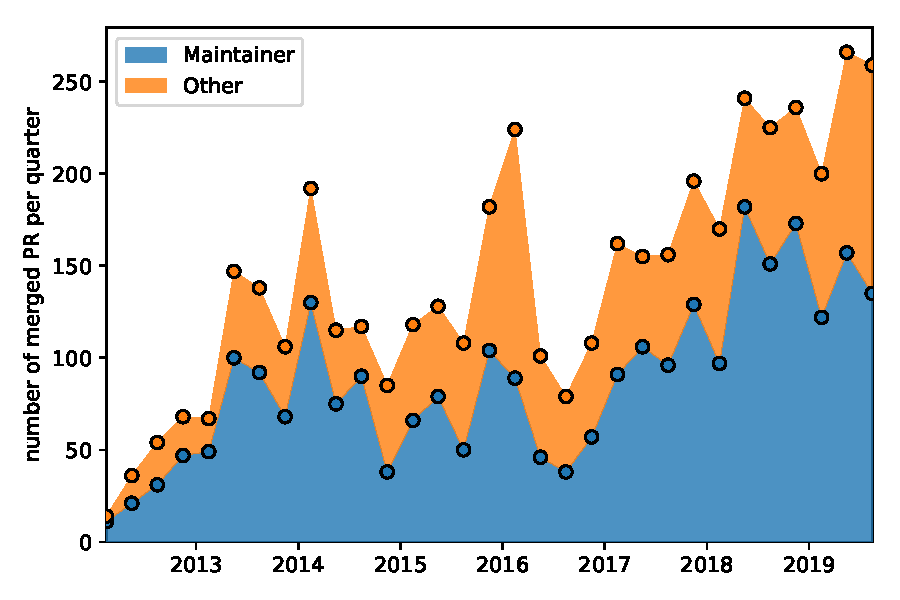
\includegraphics[width=0.9\linewidth]{scripts/PRs-using-CURRENT_MAINTAINERS.pdf}
    \caption{Number of pull requests merged into the NumPy master branch for each
        quarter since 2012. The total number of PRs is indicated with the
        lower blue area showing the portion contributed by current or previous
        maintainers.}\label{fig:prs-over-time}
\end{figure}



\subsection*{Community calls}

The massive number of scientific Python packages that
built on NumPy meant that it had an unusually high need for stability.
So to guide our development we formalized the feature proposal process, and
constructed a development roadmap with extensive input and feedback from the
community.


Weekly community calls alternate between triage and
higher level discussion.  The calls not only involve developers from
the community, but provide a venue for vendors and other external
groups to provide input.  For example, after Intel produced a forked
version of NumPy, one of their developers joined a call to discuss
community concerns.

\subsection*{NumPy enhancement proposals}

Given the complexity of the codebase and the massive number of projects depending
on it, large changes require careful planning and substantial work.
NumPy Enhancement Proposals (NEPs) are modeled after
Python Enhancement Proposals (PEPs) for ``proposing major new
features, for collecting community input on an issue, and for
documenting the design decisions that have gone into
Python''\footnote{\url{https://numpy.org/neps/nep-0000.html}}.
Since then there have been 19 proposed NEPS---6 have been implemented,
4 have been accepted and are being implemented, 4 are under
consideration, 3 have been deferred or superseded, and 2 have been rejected
or withdrawn.


\subsection*{Central role}

NumPy plays a central role in building and standardizing much of the scientific
Python community infrastructure.
The docstring standard mentioned in the history section is now widely adopted.
We are also now using the NEP system as a way to help coordinate the larger
scientific Python community.
% https://numpy.org/neps/nep-0029-deprecation_policy.html
For example, in NEP 29, we recommend, along with leaders from various other
projects, that all projects across the Scientific Python ecosystem adopt a
common ``time window-based'' policy for support of Python and NumPy versions.
This standard will simplify downstream project and release planning.

\subsection*{Wheels build system}

A Python \emph{wheel}\cite{PEP427} is a standard file format for
distributing Python libraries.  In addition to Python code, a
wheel may include compiled C extensions and other binary data.
This is important, because many libraries, including NumPy,
require a C compiler and other build tools to build the software
from the source code, making it difficult for many users to install
the software on their own.  The introduction of wheels to the Python
packaging system has made it much easier for users to install
precompiled libraries.

A GitHub repository containing scripts to build NumPy wheels has
been configured so that a simple commit to the repository triggers
an automated build system that creates NumPy wheels for several
computer platforms, including Windows, Mac OSX and Linux.  The wheels
are uploaded to a public server and made available for anyone to use.
This system makes it easy for users to install precompiled versions
of NumPy on these platforms.

The technology that is used to build the wheels evolves continually.
At the time this paper is being written, a key component is the
\code{multibuild} suite of tools developed by Matthew Brett and
other developers\cite{multibuild}.  Currently, scripts using
\code{multibuild} are written for the continuous integration
platforms Travis-CI (for Linux and Mac OSX) and Appveyor
(for Windows).

\subsection*{Recent technical improvements}

With the recent infusion of funding and a clear process for coordinating with
the developer community, we have been able to tackle a number of important
large scale changes.
We highlight two of those below, as well as changes made to our testing
infrastructure to support hardware platforms used in large scale computing.

\subsection*{Array function protocol}

A vast number of projects are built on NumPy;
these projects are consumers of the NumPy API.
Over the last several years, a growing number of projects are providers of
a \emph{NumPy-like API} and array objects targeting audiences with specialized
needs beyond NumPy's capabilities.
For example, the NumPy API is implemented by several popular tensor computation
libraries including CuPy\footnote{\url{https://cupy.chainer.org/}},
JAX\footnote{\url{https://jax.readthedocs.io/en/latest/jax.numpy.html}},
and Apache MXNet\footnote{\url{https://numpy.mxnet.io/}}.
PyTorch\footnote{\url{https://pytorch.org/tutorials/beginner/blitz/tensor\_tutorial.html}}
and Tensorflow\footnote{\url{https://www.tensorflow.org/tutorials/customization/basics}}
provide tensor APIs with NumPy-inspired semantics.
It is also implemented in packages that support sparse arrays
such as \code{scipy.sparse} and \code{pydata.sparse}.
Another notable example is Dask, a library for parallel computing in
Python.  Dask adopts the NumPy API and therefore presents a familiar
interface to existing NumPy users, while adding powerful abilities to
parallelize and distribute tasks.

The multitude of specialized projects creates the difficulty that consumers
of these NumPy-like APIs write code specific to a single project and do not support
all of the above array providers.
This is a burden for users relying on the specialized array-like, since
a tool they need may not work for them.
It also creates challenges for end-users who need to transition
from NumPy to a more specialized array.
The growing multitude of specialized projects with NumPy-like APIs threatened
to again fracture the scientific Python community.

To address these issues NumPy has the goal of providing the fundamental
API for \emph{interoperability} between the various NumPy-like APIs.
An earlier step in this direction was the implementation of the
\code{\_\_array\_ufunc\_\_} protocol in NumPy 1.13, which enabled interoperability
for most mathematical functions.\cite{NEP13}
In 2019 this was expanded more generally with the inclusion of the
\code{\_\_array\_function\_\_} protocol into NumPy~1.17.
These two protocols allow providers of array objects to be interoperable
with the NumPy API: their arrays work correctly with almost all NumPy functions.\cite{NEP18}
For the users relying on specialized array projects it means that even though
much code is written specifically for NumPy arrays and uses the NumPy API as
\code{import numpy as np}, it can nevertheless work for them.
For example, here is how a CuPy GPU array can be passed through NumPy for
processing, with all operations being dispatched back to CuPy:

\begin{lstlisting}
import numpy as np
import cupy as cp

x_gpu = cp.array([1, 2, 3])
y = np.sum(x_gpu)  # Returns a GPU array
\end{lstlisting}

Similarly, user defined functions composed using NumPy can now be
applied to, e.g., multi-node distributed Dask arrays:

\begin{lstlisting}
import numpy as np
import dask.array as da


def f(x):
    """Function using NumPy API calls"""
    y = np.tensordot(x, x.T)
    return np.mean(np.log(y + 1))


x_local = np.random.random([10000, 10000])  # random local array
x_distr = da.random.random([10000, 10000])  # random distributed array

f(x_local)  # returns a NumPy array
f(x_distr)  # works, returns a Dask array
\end{lstlisting}

\subsection*{Random number generation}

The NumPy \code{random} module provides pseudorandom numbers from a wide range of
distributions. In legacy versions of NumPy, simulated random values are produced
by a \code{RandomState} object that: handles seeding and state initialization;
wraps the core pseudorandom number generator based on a Mersenne Twister
implementation\footnote{to be precise, the standard 32-bit version of MT19937};
interfaces with the underlying code that transforms random bits into
variates from other distributions; and supplies a singleton instance exposed in
the root of the random module.

The \code{RandomState} object makes a compatibility guarantee so that a fixed
seed and sequence of function calls produce the same set of values. This
guarantee has slowed progress since improving the underlying code requires
extending the API with additional keyword arguments. This guarantee continues to
apply to \code{RandomState}.

NumPy 1.17 introduced a new API for generating random numbers that use a more
flexible structure that can be extended by libraries or end-users. The new API
is built using components that separate the steps required to generate random
variates. Pseudorandom bits are generated by a bit generator. These bits are
then transformed into variates from complex distributions by a generator.
Finally, seeding is handled by an object that produces sequences of high-quality
initial values.

Bit generators are simple classes that manage the state of an underlying
pseudorandom number generator. NumPy ships with four bit generators. The default
bit generator is a 64-bit implementation of the Permuted Congruential Generator
\cite{pcg64} (\code{PCG64}). The three other bit generators are a 64-bit version
of the Philox generator\cite{random123} (\code{Philox}), Chris Doty-Humphrey's
Small Fast Chaotic generator\cite{practrand} (\code{SFC64}), and the 32-bit
Mersenne Twister\cite{mt19937} (\code{MT19937}) which has been used in older
versions of NumPy.\footnote{The
\href{https://github.com/bashtage/randomgen}{randomgen project} supplies a wide
range of alternative bit generators such as a cryptographic counter-based
generators (\code{AESCtr}) and generators that expose hardware random number
generators (\code{RDRAND})\cite{randomgen}.} Bit generators provide
functions, exposed both in Python and C, for generating random integer
and floating point numbers.

The \code{Generator} consumes one of the bit generators and produces variates
from complicated distributions. Many improved methods for generating random
variates from common distributions were implemented, including the Ziggurat
method for normal, exponential and gamma variates\cite{ziggurat}, and Lemire's
method for bounded random integer generation\cite{lemire}. The \code{Generator}
is more similar to the legacy \code{RandomState}, and its API is substantially
the same. The key differences all relate to state management, which has been
delegated to the bit generator. The \code{Generator} does not make the same
stream guarantee as the \code{RandomState} object, and so variates may differ
across versions as improved generation algorithms are
introduced.\footnote{Despite the removal of the compatibility guarantee, simple
reproducibility across versions is encouraged, and minor changes that do not
produce meaningful performance gains or fix underlying bug are not generally
adopted.}

Finally, a \code{SeedSequence} is used to initialize a bit generator. The seed
sequence can be initialized with no arguments, in which case it reads entropy
from a system-dependent provider, or with a user-provided seed. The seed
sequence then transforms the initial set of entropy into a sequence of
high-quality pseudorandom integers, which can be used to initialize multiple bit
generators deterministically. The key feature of a seed sequence is that
it can be used to spawn child \code{SeedSequence}s which allow to initialize
multiple distinct bit generators.
% Of course there is a diminishing chance of collisions...
% Only found http://www.pcg-random.org/posts/developing-a-seed_seq-alternative.html
% as a reference for seed sequence, it would be nice to cite something.
This capability allows a seed sequence to facilitate large distributed applications
where the number of workers required is not known. The sequences generated from
the same initial entropy and spawns are fully deterministic to ensure
reproducibility.

The three components are combined to construct a complete random number
generator.

\begin{lstlisting}
from numpy.random import (
    Generator,
    PCG64,
    SeedSequence,
)

seq = SeedSequence(1030424547444117993331016959)
pcg = PCG64(seq)
gen = Generator(pcg)
\end{lstlisting}

This approach retains access to the seed sequence which can then be
used to spawn additional generators.

\begin{lstlisting}
children = seq.spawn(2)
gen_0 = Generator(PCG64(children[0]))
gen_1 = Generator(PCG64(children[1]))
\end{lstlisting}

While this approach retains complete flexibility, the method
\code{np.random.default\_rng} can be used to instantiate a \code{Generator} when
reproducibility is not needed.

The final goal of the new API is to improve extensibility. \code{RandomState} is
a monolithic object that obscures all of the underlying state and functions. The
component architecture is one part of the extensibility improvements. The
underlying functions (written in C) which transform the output of a bit
generator to other distributions are available for use in CFFI. This allows the
same code to be run in both NumPy and dependent that can consume CFFI, e.g.,
Numba. Both the bit generators and the low-level functions can also be used in C
or Cython code.\footnote{As of 1.18.0, this scenario requires access to the
NumPy source. Alternative approaches that avoid this extra step are being
explored.}

\subsection*{Testing on multiple architectures}

At the time of writing the two fastest supercomputers in the
world, Summit and Sierra, both have IBM POWER9 architectures
\cite{top500nov2019}. In late 2018, Astra, the first ARM-based
supercomputer to enter the TOP500 list, went into production\cite{
astra-wiki}. Furthermore, over 100 billion ARM processors have been
produced as of 2017\cite{arm-architecture}, making it the most 
widely used instruction set architecture in the world.

Clearly there are motivations for a large scientific computing
software library to support POWER and ARM architectures. We've extended
our continuous integration (CI) testing to include \texttt{ppc64le}
(POWER8 on Travis CI) and ARMv8 (on Shippable service). We also test
with the s390x architecture (IBM Z CPUs on Travis CI) so that we
can probe the behavior of our library on a big-endian machine.
This satisfies one of the major components of
improved CI testing laid out in a version of our roadmap
\cite{numpy-roadmap}---specifically, ``CI for more exotic
platforms."

PEP 599\cite{PEP599} lays out a plan for new Python binary wheel
distribution support, \texttt{manylinux2014}, that adds
support for a number of architectures supported by the CentOS
Alternative Architecture Special Interest Group, including
ARMv8, ppc64le, as well as s390x. We are thus well-positioned
for a future where provision of binaries on these architectures
will be expected for a library at the base of the ecosystem.
